\documentclass{article}

\usepackage{Sweave}
\begin{document}
\Sconcordance{concordance:Homework2.tex:Homework2.Rnw:%
1 2 1 1 0 7 1 1 3 2 0 2 1 1 3 1 0 1 1 1 15 13 0 1 9 7 0 1 17 15 0 1 8 6 %
0 1 2 4 0 1 2 1 1 1 2 1 0 1 1 1 2 1 1 1 5 4 0 1 7 5 0 2 1 1 2 1 0 1 2 1 %
0 1 2 1 0 1 8 6 0 1 1 5 0 1 3 3 1}


\begin{center}
{\bf\Large Practice 1}
\end{center}

\section*{Question 1}
\begin{Schunk}
\begin{Sinput}
> #set workspace and read file
> setwd("/Users/xinhuang/Google Drive/CSC 522 R Language Programming /Homework2")
> sfData <- read.csv("AirQualitySanFranciscoData.csv", header = TRUE)
> sdData <- read.csv("AirQualitySanDiegoData.csv", header = TRUE)
> # set layout
> mat <- matrix(1 : 4, nrow = 2)
> layout(mat)
> with(sfData, {
+     plot(Year, ExceedStateLevelDays1.hr, col = "red", ylim = c(0, 100), 
+          type = "b", ylab = "Number of Days over Standard", 
+          pch = 20, lty = 2)
+     points(Year, ExceedStateLevelDays8.hr, col = "yellow", 
+            type = "b", pch = 20, lty = 3)
+     points(Year, ExceedNationalLevelDays8.hr, col = "green", 
+            type = "b", pch = 20, lty = 4)
+     title(main = "San Francisco Air Quality")
+     legend("topright", 
+            c("State Days 1 hour", "State Days 8 hours", "National Level 8 hours"),
+            col = c("red", "yellow", "green"),
+            pch = 1, cex = 0.5, title = "Over standard")
+ })
> with(sfData, {
+     plot(Year, MaxConcentration1.hr, col = "cyan", ylim = c(0.04, 0.17), 
+          type = "b", ylab = "Maximum Concentration", pch = 20, lty = 2)
+     points(Year, MaxConcentration8.hr, col = "blue", 
+            type = "b", pch = 20, lty = 3)
+     legend("topright", c("Max 1 hour", "Max 8 hour"),
+            col = c("cyan", "blue"), pch = 1, cex = 0.5, title = "ppm")
+ })
> with(sdData, {
+     plot(Year, ExceedStateLevelDays1.hr, col = "red", ylim = c(0, 100), 
+          type = "b", ylab = "Number of Days over Standard",
+          pch = 20, lty = 2)
+     points(Year, ExceedStateLevelDays8.hr, col = "yellow",
+            type = "b", pch = 20, lty = 3)
+     points(Year, ExceedNationalLevelDays8.hr, col = "green", 
+            type = "b", pch = 20, lty = 4)
+     title(main = "San Diego Air Quality")
+     legend("topright", 
+            c("State Days 1 hour", 
+              "State Days 8 hours", 
+              "National Level 8 hours"),
+            col = c("red", "yellow", "green"), pch = 1, 
+            cex = 0.5, title = "Over standard")
+ })
> with(sdData, {
+     plot(Year, MaxConcentration1.hr, col = "cyan", ylim = c(0.04, 0.17), 
+          type = "b", ylab = "Maximum Concentration", pch = 20, lty = 2)
+     points(Year, MaxConcentration8.hr, col = "blue", type = "b", pch = 20, lty = 3)
+     legend("topright", c("Max 1 hour", "Max 8 hour"),
+            col = c("cyan", "blue"), pch = 1, cex = 0.5, title = "ppm")
+ })
> mtext("Main title", line=2, font=2, cex=1.2, outer = TRUE)
\end{Sinput}
\end{Schunk}
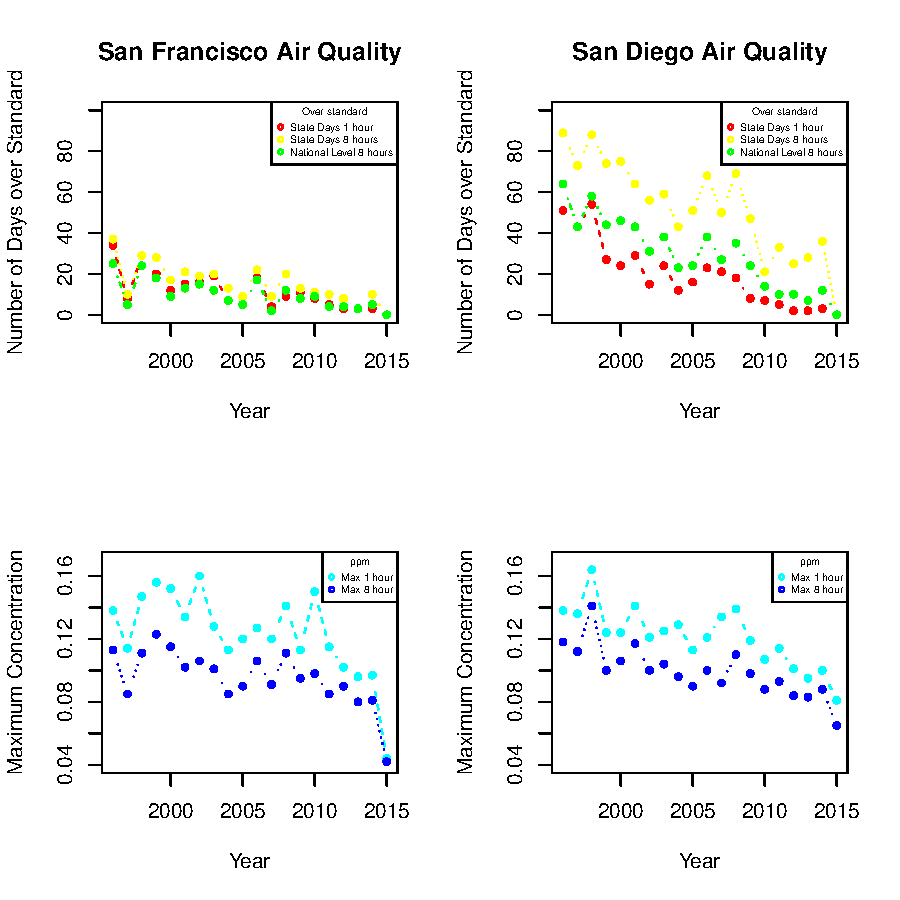
\includegraphics{Homework2-001}

\section*{Question 2}
\begin{Schunk}
\begin{Sinput}
> mat <- matrix(1 : 2, nrow = 2)
> layout(mat)
> myState <- as.data.frame(state.x77)
> d <- density(myState$Area)
> axisV <- as.integer(c(min(myState$Area),
+                       mean(myState$Area),
+                       myState[rownames(myState)== "Texas",
+                               colnames(myState)=="Area"],
+                       max(myState$Area))) 
> plot(d, col = "red", lwd = 2,
+     xlim=c(min(myState$Area),max(myState$Area)),
+     xlab = "Land Area in Square Miles",
+     ylab = "Density",
+     xaxt = "n",
+     main = "Probability Density Plot \n State Land Area in Square Miles")
> axis(1, at = axisV, labels = axisV) 
> abline(v=mean(myState$Area),col = "black", lty = 5) 
> text(2 * mean(myState$Area) + 20000, 11e-06,
+      paste("mean = ",round(mean(myState$Area), digits=0)))
> text(myState$Area[rownames(myState)=="Alaska"]-85000, 8e-06,
+      paste("Alaska Area = \n",myState$Area[rownames(myState)=="Alaska"])) 
> text(myState$Area[rownames(myState)=="Texas"]-3000, 8e-06,
+      paste("Texas Area = \n",myState$Area[rownames(myState)=="Texas"]))
> hist(myState$Area, 
+      breaks= 50, 
+      col="red",
+      xaxt = "n",
+      xlim=c(min(myState$Area),max(myState$Area)),
+      xlab = "Land Area in Square Miles",
+      main = "Histogram of State Land Area in Square Miles")
> axis(1, at = axisV, labels = axisV) 
> 
\end{Sinput}
\end{Schunk}
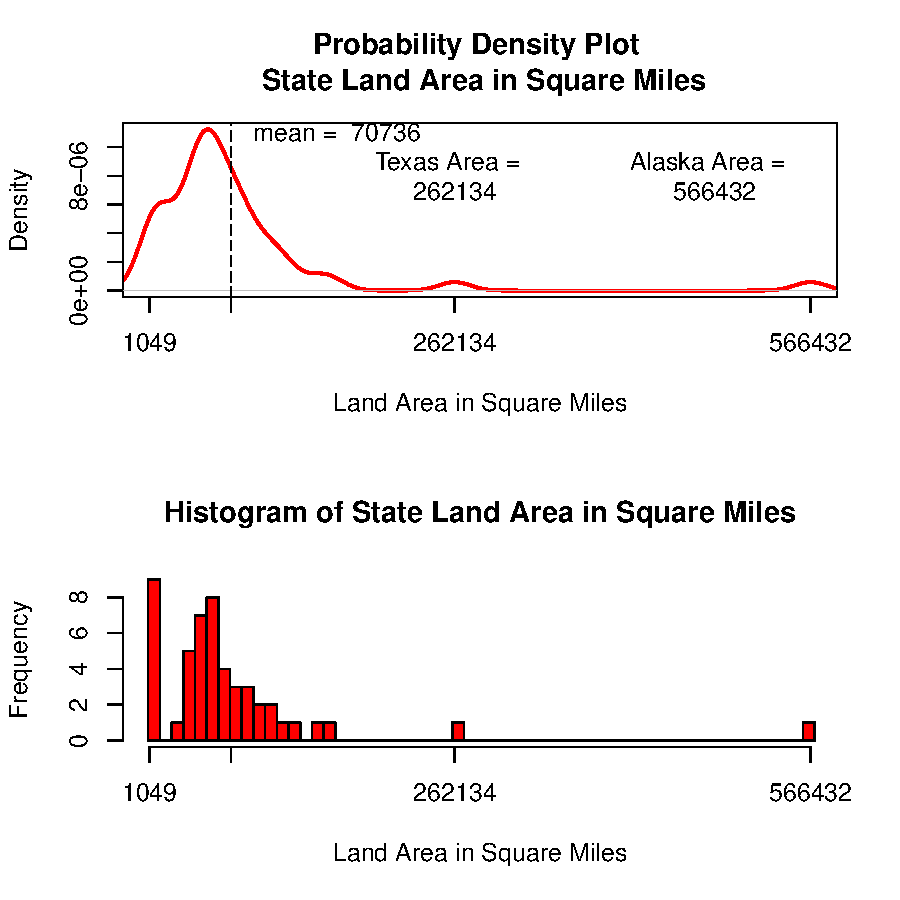
\includegraphics{Homework2-002}



\end{document}
